\section{Aproximação de Derivadas Parciais por Diferenças Finitas}

A derivada parcial

\[
 f_{,x} = \frac{\partial f\,(x,\,y)}{\partial x} \quad \mbox{em} \quad (x,y) = (x_{0},y_{0})
\]

pode ser deduzida fixando-se \esp{y = y_{0}} e considerando-se \esp{f(x,y_{0})} como uma função de uma variável. Assim, as aproximações de \esp{f_{,x}} por diferenças finitas são:

\[
 f_{,x} \approx \frac{f\,(x_0 + \Delta x,\,y_0) - f\,(x_0,\,y_0)}{\Delta x} \qquad Forward
\]

\[
 f_{,x} \approx \frac{f\,(x_0 + \Delta x,\,y_0) - f\,(x_0 - \Delta x,\,y_0)}{2\,\Delta x} \qquad Central
\]

\[
 f_{,x} \approx \frac{f\,(x_0,\,y_0) - f\,(x_0 - \Delta x,\,y_0)}{\Delta x} \qquad Backward
\]

Diferenças centradas das derivadas parciais $f_{,xx}$, $f_{,yy}$ e $f_{,xy}$:

\[
 f_{,xx} = \frac{\partial^2}{\partial x^2} \, f \approx \frac{f\,(x_0 + \Delta x,\, y_0) - 2\,f\,(x_0,\,y_0) + f\,(x_0 - \Delta x,\,y_0)}{\Delta x^2}
\]

\[
 f_{,yy} = \frac{\partial^2}{\partial y^2} \, f \approx \frac{f\,(x_0,\, y_0 + \Delta y) - 2\,f\,(x_0,\,y_0) + f\,(x_0,\, y_0 - \Delta y)}{\Delta y^2}
\]

\[
 \begin{array}{ll}
  f_{,xy} = \displaystyle \frac{\partial^2}{\partial x \, \partial y} \, f & \approx \displaystyle \frac{f\,(x_0 + \Delta x,\, y_0 + \Delta y) - f\,(x_0 + \Delta x,\,y_0 - \Delta y)}{4\,\Delta x \, \Delta y} \vspace*{0.2cm} \\
   & + \displaystyle \frac{-f\,(x_0 - \Delta x,\, y_0 + \Delta y) + f\,(x_0 - \Delta x,\, y_0 - \Delta y)}{?}
 \end{array}
\]

\subsection{Solução do Problema de Dirichlet}

\textbf{Deformação de uma membrana}\\

EDP: \esp{\displaystyle \frac{\partial^2 u}{\partial x^2} + \frac{\partial^2 u}{\partial y^2} = 0} em \esp{x \in (0,\,1)} e \esp{y \in (0,\,1)} \\

C.C.:

\[
\begin{array}{l}
 u = 0 \quad \mbox{em} \quad
 \left\{
 \begin{array}{l}
  y = 1 \\
  x = 0 \\
  x = 1
 \end{array} \right. \\
 \\
 u\,(x,\,0) = sin\,(\pi \, x) \quad \mbox{com} \quad x \in [0,\,1]
\end{array}
\]

\begin{figure}[htb]
 \centering
 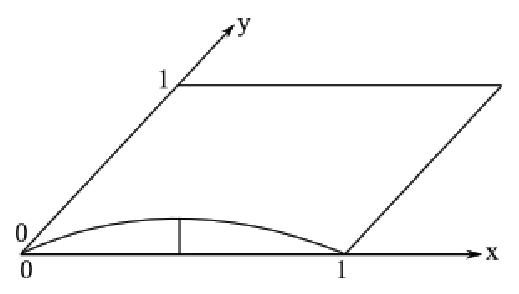
\includegraphics[scale=1.0]{capitulos/capitulo3/figuras/aprox_der_par_dif_fin1.eps}
 \caption{?}
 \label{fig:aprox_der_par_dif_fin1}
\end{figure}

\textbf{Solução:}

\begin{enumerate}
 \item Discretizar o domínio numa grade de pontos:

\begin{figure}[htb]
 \centering
 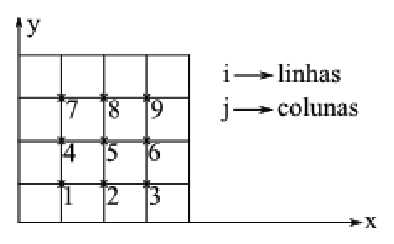
\includegraphics[scale=1.0]{capitulos/capitulo3/figuras/aprox_der_par_dif_fin2.eps}
 \caption{?}
 \label{fig:aprox_der_par_dif_fin2}
\end{figure}

\item Escreva a E.D.P. utilizando operadores diferenciais centrados no ponto \esp{(i,\,j)}:

\begin{equation}
 \label{cap3:sec4:eq1}
 \frac{\partial^2 u}{\partial x^2} = \frac{1}{h_x^2} \, (u_{i,j+1} - 2\,u_{i,j} + u_{i,j-1})
\end{equation}

\begin{equation}
 \label{cap3:sec4:eq2}
 \frac{\partial^2 u}{\partial y^2} = \frac{1}{h_y^2} \, (u_{i+1,j} - 2\,u_{i,j} + u_{i-1,j})
\end{equation}

Se \esp{h_x = h_y = h}

\begin{equation}
 \label{cap3:sec4:eq3}
 \frac{\partial^2 u}{\partial x^2} + \frac{\partial^2 u}{\partial y^2} \approx \frac{1}{h^2} \, (u_{i+1,j} + u_{i-1,j} + u_{i,j+1} + u_{i,j-1} - 4\,u_{i,j}) = 0
\end{equation}

\item Definir a célula diferencial

\[
 \begin{array}{lll}
                   & \quadricular{+1} & \vspace*{0.2cm} \\
  \quadricular{+1} & \quadricular{-4} & \quadricular{+1} \vspace*{0.2cm} \\
                   & \quadricular{+1} &
 \end{array}
\]

\item Aplicar a célula a cada ponto interior (P1 a P9):

\[
\begin{array}{l}
 P1: \\
 P2: \\
 P3: \\
 P4: \\
 P5: \\
 P6: \\
 P7: \\
 P8: \\
 P9:
\end{array}
\,
\left[
\begin{array}{rrrrrrrrr}
 -4 &  1 &  0 &  1 &  0 &  0 &  0 &  0 &  0\\
  1 & -4 &  1 &  0 &  1 &  0 &  0 &  0 &  0\\
  0 &  1 & -4 &  0 &  0 &  1 &  0 &  0 &  0\\
  1 &  0 &  0 & -4 &  1 &  0 &  1 &  0 &  0\\
  0 &  1 &  0 &  1 & -4 &  1 &  0 &  1 &  0\\
  0 &  0 &  1 &  0 &  1 & -4 &  0 &  0 &  1\\
  0 &  0 &  0 &  1 &  0 &  0 & -4 &  1 &  0\\
  0 &  0 &  0 &  0 &  1 &  0 &  1 & -4 &  1\\
  0 &  0 &  0 &  0 &  0 &  1 &  0 &  1 & -4
\end{array}
\right]
\,
\left\{
\begin{array}{l}
 u_1 \\
 u_2 \\
 u_3 \\
 u_4 \\
 u_5 \\
 u_6 \\
 u_7 \\
 u_8 \\
 u_9
\end{array}
\right\}
+
\left\{
\begin{array}{c}
 sin\,\left(\frac{\pi}{4}\right) \\
 sin\,\left(\frac{\pi}{2}\right) \\
 sin\,\left(\frac{3\,\pi}{4}\right) \\
 0 \\
 0 \\
 0 \\
 0 \\
 0 \\
 0
\end{array}
\right\}
=
\{0\}
\]

\end{enumerate}
